\documentclass[a4paper, 12pt]{article}
\usepackage{style}
\usepackage{hyperref}

%colori per tablle tabu
\definecolor{tableHeader}{RGB}{254, 61, 0}
\definecolor{tableLineOne}{RGB}{245, 245, 245}
\definecolor{tableLineTwo}{RGB}{254,204,188}
%define header tabelle tabu
\newcommand{\tableHeaderStyle}{
    \rowfont[c]{\leavevmode\color{white}\bfseries}
    \rowcolor{tableHeader}
}

\title{NormeDiProgetto}
\author{Cyber13}
\date{March 2019}

\begin{document}
	\begin{titlepage}
		\centering Università degli Studi di Padova
		\line(1,0){350}\\
		\vspace{1.2cm}
		\logo
		\vspace{1.0cm}
		\centering{\bfseries\LARGE NORME DI PROGETTO \\}
		\vspace{0.5cm}
		\centering{\slshape\large Gruppo Cyber13 - Progetto P2PCS\\}
		\vspace{0.5cm}
		\centering{\bfseries Informazioni sul documento \\}
		\line(1,0){240}\\
		% compilare i campi per ogni documento
		\begin{tabular}{r|l}
			{\textbf{Versione}} 			& 1.0.0\\
			{\textbf{Data Redazione}} 	& 09/03/2019\\	% aggiornare la data
			{\textbf{Responsabili}} 	& Matteo Squeri \\ & Andrea Casagrande \\	% aggiornare la data
			{\textbf{Redazione}} 		 & Andrea Casagrande \\& Elena Pontecchiani \\ & Ilaria Rizzo \\ 
			{\textbf{Verifica}} 			& Fabio Garavello \\ & Matteo Squeri\\  & Daniel Mirel Bira\\ 
			{\textbf{Approvazione}} 		& Andrea Casagrande\\
			{\textbf{Uso}} 				& Interno\\
			{\textbf{Destinatari}} 	& Cyber13\\ & Prof. Tullio Vardanega\\ & Prof. Riccardo Cardin\\
			{\textbf{Mail di contatto}} 	& swe.cyber13@gmail.com\\
		\end{tabular}\\
	\end{titlepage}

	\newpage
		\subfile{DiarioModificheNdP.tex}
	\newpage
		\tableofcontents
        	\newpage
	    	\listoffigures
	    	\newpage
        	\section{Introduzione}
                \subsection{Scopo del documento}
Il documento ha lo scopo di fissare precise norme che regolamenteranno
l’intero svolgimento del progetto. \\
Tutti i membri del team sono obbligati a visionare tale documento e a sottostare alle norme ivi descritte.
Le norme contenute nel documento si occupano di regolamentare i diversi processi all'interno del progetto. La regolamentazione tramite norme permette di sviluppare prodotti coerenti e consistenti tra i vari componenti del gruppo e facilitare l’esecuzione delle  operazioni di verifica.
In particolare le norme si occuperanno di regolamentare:
    \begin{itemize}
        \item Le modalità di interazione tra i membri del team e le persone esterne al team;
        \item L'organizzazione del team: verranno definiti e assegnati ruoli ai membri del team. Per ogni ruolo verranno identificate determinate mansioni;
        \item Le convenzioni tipografiche e le modalità di stesura delle documentazioni;
        \item Gli ambienti di sviluppo, il \citgl{repository} e il \citgl{ticketing};
    \end{itemize}

Nel caso in cui ve ne sia necessità, ogni membro del team potrà contattare il
\citgl {Project Manager} per suggerire eventuali cambiamenti
\subsection{Scopo del prodotto}
Lo scopo del prodotto è quella di realizzare un'applicazione \citgl{Android} che implementi un servizio di car sharing \citgl{peer-to-peer}.

\subsection{Glossario}
Onde evitare ambiguità o incomprensioni di natura lessicale, si allega il \G.
All'interno del documento saranno presenti parole di ambito specifico, uso raro che potrebbero creare incomprensioni. Per una maggiore leggibilità tali parole sono riconoscibili all'interno dei vari documenti in quanto scritte in corsivo e con un 'g' a pedice tra barre orizzontali (per esempio \citgl{Glossario})
Nel caso esistano più ripetizioni di una stessa parola del glossario all'interno di uno stesso paragrafo, la dicitura con la lettera 'g' a pedice sarà inserita solo la prima volta che la parola comparirà.
Il comando LaTeX da utilizzare per contrassegnare un termine da glossario all’interno dei documenti è \textbackslash \textit{citgl}\{..\}.



\subsection{Riferimenti}
    \subsubsection {Riferimenti normativi}
        \begin{itemize}
        \item \NdP;
    \end{itemize}
    \subsubsection {Riferimenti informativi}
        \begin{itemize}
        \item \AdR;
        \item \PdP;
        \item \PdQ;
        \item \SdF;
        \item Sito del corso di Ingegneria del Software: \\ \url{https://www.math.unipd.it/~tullio/IS-1/2018/}
        \item  Software Engineering - Ian Sommerville - 10th Edition;
        \item Materiale suggerito dalla proponente:
        \begin{itemize}
            \item Materiale \citgl{MVP}:
           \\ \href{https://medium.com/@cervonefrancesco/model-view-presenter-android-guidelines-94970b430ddf}{https://model-view-presenter-android-guidelines}
            \item Materiale Testing e \citgl{Refactoring}
           \\ \url{https://www.youtube.com/watch?v=_NnElPO5BU0}
        \end{itemize}
        
    \end{itemize}

                \newpage
            \section{Processi primari}
                \subsection{Processo di fornitura}
 \subsubsection{Scopo}
In  questa  sezione  vengono sancite precise norme per quanto riguarda il rapporto di fornitura con la proponente \citgl{GaiaGo} e  dei committenti  Prof. Tullio Vardanega e Prof. Riccardo Cardin nell’ambito della progettazione, sviluppo e consegna del prodotto P2PCS. \\
Le norme  ivi trattate sono tassative e i membri del gruppo Cyber13  sono tenuti a rispettarle al fine di proporsi e diventare fornitori.

\subsubsection{Aspettative}
Il gruppo intende mantenere un costante dialogo con il proponente per avere un riscontro efficace sul lavoro svolto.\\
Nel corso dell'intero progetto il team Cyber13 si auspica di instaurare con la committente GaiaGo, nel particolare con il referente Filippo Pretto, un rapporto di collaborazione al fine di:
    \begin{itemize}
        \item Determinare come adempire appieno ai requisiti fissati dal proponente;
        \item Determinare vincoli sui processi e i requisiti;
        \item Eseguire una stima dei costi;
        \item Concordare la qualifica del prodotto.
    \end{itemize}


\subsubsection{Attività}
    \paragraph{Studio di fattibilità}
    ~\\
    In seguito alla formazione ufficiale dei gruppi del secondo lotto, avvenuta in data 4 Marzo 2019, è stata convocata una riunione interna al gruppo per discutere in merito ai vari capitolati disponibili per lo svolgimento del progetto, presentati in data 16 Novembre 2018.\\
    Una volta stabilita la scelta del capitolato per il quale proporsi come fornitori, gli analisti hanno condotto un’ulteriore e approfondita attività di analisi dei rischi e delle opportunità culminata con la redazione del documento \SdF .
    Tale documento include le motivazioni che hanno portato il gruppo Cyber13 a
    proporsi come fornitore per il prodotto indicato e riporta per ciascun capitolato:
    \begin{itemize}
        \item \textbf{Informazioni sul capitolato}: In cui vengono riportati nome del progetto, azienda proponente e i committenti.
        \item \textbf{Descrizione}: All'interno della quale viene descritto brevemente cosa il progetto richiede.
        \item \textbf{Studio del dominio}: Nel quale vengono indicati i domini applicativi e tecnologici del capitolato.
        \item \textbf{Esito finale}: Dove sono riportati aspetti positivi, fattori di rischio e conclusione finale del gruppo in merito al capitolato.
    \end{itemize}
    
    \paragraph{Piano di progetto}
    ~\\
    Il responsabile avrà il compito di redigere il documento \PdP. Tale documento formale descrive:
    \begin{itemize}
        \item Gli obiettivi del progetto.
        \item Le attività da svolgere per adempire agli obiettivi rispettando i requisiti fissati. Attraverso l'attività di pianificazione si organizzano le diverse attività da svolgere con precise tempistiche da rispettare.
        \item Le risorse coinvolte (in termini di personale e di tecnologie impiegate).
        \item I costi previsti, che vengono stabiliti attraverso il preventivo e il consuntivo. Sulla base della pianificazione si stima la quantità di lavoro necessaria per ogni fase, proponendo così un preventivo per il costo totale del progetto. Alla fine di ogni attività si redige inoltre un consuntivo di periodo per tracciare l’andamento rispetto a quanto preventivato;
        \item I rischi potenziali attraverso l'analisi dei rischi. Si analizzano nel dettaglio i rischi che potrebbero insorgere nel corso del progetto e i modi per affrontarli, capendo la probabilità che essi accadano e il livello di gravità ad essi associato.
    \end{itemize}
    
    \paragraph{Piano di qualifica}
     I verificatori dovranno scegliere una strategia da adottare per la \citgl{verifica} e la \citgl{validazione} del materiale prodotto dal gruppo. Il documento dovrà contenere:
     \begin{itemize}
         \item \textbf{Visione generale delle strategie di verifica}: Si stabiliscono le procedure di controllo sulla qualità di processo e di prodotto, tenendo in considerazione le risorse a disposizione.
         \item \textbf{Misure e metriche}: Si devono stabilire delle metriche oggettive per i documenti, i processi e il software.
         \item \textbf{Gestione della revisione}: Si devono stabilire le modalità di comunicazione delle anomalie e le procedure di controllo per la qualità di processo.
         \item \textbf{Pianificazione del collaudo}: Si devono definire nel dettaglio le metodologie di collaudo del prodotto realizzato.
         \item \textbf{Resoconto delle attività di verifica}: Alla fine di ogni attività si devono riportare le metriche calcolate e un resoconto sulla verifica di tale attività.
     \end{itemize}















                
\subsection{Processo di sviluppo}
\subsubsection{Scopo}
Il processo di sviluppo contiene tutte le attività di analisi, design, codifica, integrazione ed installazione relative al prodotto da sviluppare. Di seguito sono raccolte le linee guida che verranno utilizzate dei membri del gruppo nelle principali attività di questo processo. \\
Pertanto il processo si compone delle seguenti attività:
    \begin{itemize}
        \item Analisi dei requisiti;
        \item Progettazione;
        \item Codifica.
    \end{itemize}


\subsubsection{Aspettative}
Gli obiettivi perseguiti in fase di sviluppo sono i seguenti:
    \begin{itemize}
        \item Realizzare un prodotto finale conforme alle richieste del proponente;
        \item Realizzare un prodotto finale soddisfacente i test di verifica e di validazione.
        
    \end{itemize}



\subsubsection{Attività}
    \paragraph{Analisi dei requisiti}
        \subparagraph{Scopo}
         ~\\
         L'analisi dei requisiti è un documento ad uso esterno, il cui compito è fornire una descrizione completa di tutti i 
         \citgl{requisiti} individuati in fase di analisi dagli analisti e dei casi d'uso riguardanti il progetto \citgl{P2PCS}. \\
         Le informazioni estrapolate sono state ottenute dall'esposizione del capitolato e soprattutto attraverso incontri con il referente dell'azienda proponente. \\
         In seguito sono elencate le norme che riguardano i requisiti esposti nel documento \AdR, al fine di evitare ambiguità o difformità di natura formale. \\
         La tecnica utilizzata per l’analisi e la ricerca dei requisiti è quella dei casi d’uso.
         \subparagraph{Aspettative}
         ~\\
         L'obiettivo dell'attività è la creazione della documentazione formale contenente tutti i requisiti richiesti dal proponente.
        \subparagraph{Classificazione dei requisiti}
        ~\\
        Ad ogni requisito individuato in fase di analisi viene identificato un codice univoco, espresso nel seguente formato:\\
        \begin{center}
        R[Priorità][Tipo][Codice]
        \end{center}
        \\
        Dove:
        \begin{itemize}
            \item \textbf{R}: abbreviazione di requisito.
            \item \textbf{Priorità}: Indica l'importanza di un requisito, e può assumere i seguenti valori (mutuamente esclusivi ed espressi in ordine decrescente di importanza):
                \begin{itemize}
                    \item C: Dall'inglese 'compulsory', che significa obbligatorio, indica un requisito irrinunciabile per il committente.
                    \item D: Dall'inglese 'desirable', desiderabile. Requisito auspicabile ma non strettamente necessario.
                   
                    
                \end{itemize}
            \item \textbf{Tipo}: Indica la classificazione del vincolo. Può assumere i seguenti valori:
                \begin{itemize}
                    \item F: Indica un requisito funzionale, ovvero la definizione di una funzione/caratteristica che deve essere implementata in un sistema.  Questa tipologia di requisiti descrivono quindi come il software reagisce a situazioni ed input particolari;
                    \item Q: Indica un requisito di qualità. Includono i requisiti di
                    \citgl{efficacia}, \citgl{efficienza}
                     e i requisiti per garantire la qualità del prodotto;
                    \item V: Indica requisiti di vincolo imposti dalla proponente GaiaGo.
                \end{itemize}
            
            \item \textbf{Codice}: Numero intero univoco e incrementale di tre cifre associato al particolare requisito sulla base dell'ordine in cui compare nella struttura del documento.
        \end{itemize}
        
    
    \subparagraph{Classificazione dei casi d'uso}
    ~\\
    Gli Analisti hanno inoltre il compito di individuare i diversi \citgl{Casi d'uso}, elencandoli attraverso una strategia \citgl{Top down}, ovvero partendo dal generale e in seguito scendendo nel particolare. \\
    I casi d'uso hanno lo scopo di descrivere scenari di interazione tra utenti e un sistema. Ciascun caso d'uso presente nel documento di Analisi dei Requisiti sarà corredato delle seguenti informazioni:
        \begin{itemize}
            \item \textbf{Codice identificativo e nome}: Ogni caso d'uso è identificato da un codice univoco strutturato nel seguente modo:
                \begin{center}
                    UC [Codice Padre].[Codice Figlio]-Nome
                \end{center} 
                \\
                Dove:
                    \begin{itemize}
                        \item UC: Indica "User case", caso d'uso in inglese;
                        \item Codice Padre: Numero intero;
                        \item Codice Figlio: Uno o più numeri interi che specificano l'annidamento del caso;
                        \item Nome del caso d'uso.
                    \end{itemize}
                    
            \item \textbf{Attori}: Indica gli attori principali (obbligatoriamente) e secondari (opzionalmente, se esistono) del caso d'uso.
            \item \textbf{Scopo e descrizione}: Riporta una breve descrizione del caso d’uso.
            \item \textbf{Scenario principale}: Descrizione  di ciò che il caso d’uso vuole modellare, indicando ogni azione che ne fa parte.
            \item \textbf{Precondizione}: Specifica le condizioni che sono identificate come vere prima del verificarsi degli eventi del caso d’uso.
            \item \textbf{Postcondizione}: Specifica le condizioni che sono identificate come vere dopo il verificarsi degli eventi del caso d’uso.
            \item \textbf{Scenari alternativi (opzionale)}: Descrizione di una possibilità alternativa allo scenario principale.
            \item \textbf{Inclusioni (opzionale)}: Usate per non descrivere più volte lo stesso flusso di eventi, inserendo il comportamento comune in un caso d’uso a parte.
            \item \textbf{Estensioni (opzionale)}: Descrivono i casi d’uso che non  fanno parte del flusso principale degli eventi, allo stesso modo di quanto  descritto in “Scenario principale”.
        \end{itemize}
   Faremo inoltre uso dei \citgl{diagrammi dei casi d'uso} , descritti nel linguaggio \citgl{UML 2.0}, per mettere in evidenza gli attori ed i servizi del sistema. 
    
    
    
    

\paragraph{Progettazione}
    \subparagraph{Scopo}
    ~\\
    L'attività di progettazione precede la fase di realizzazione ed è svolta dai progettisti. Essi hanno il compito di sviluppare e documentare una visione architetturale ad alto livello del prodotto identificando componenti chiare, riusabili e coese rimanendo nei costi fissati. Nel processo di descrizione dell' \citgl{archittettura} saranno fissate le componenti che andranno a costituire il sistema, con relative dipendenze e interazioni tra le loro istanze. I progettisti definiranno inoltre le interfacce necessarie a consentire l'interazione tra componenti e i \citgl{design pattern} da utilizzare.\\
    Durante questa attività è molto importante che i progettisti si confrontino con l’azienda proponente, allo scopo di ottenere feedback e consigli. L’attività di progettazione è documentata nella
    \citgl{Technology Baseline} e nella \citgl{Product Baseline} che saranno consegnati rispettivamente alla Revisione di Progettazione e alla Revisione di Qualifica.\\
    L’architettura definita avrà i seguenti obiettivi:
        \begin{itemize}
            \item Soddisfare i requisiti individuati in fase di analisi e riportati nel documento \AdR e adattarsi in caso questi evolvano o se ne aggiungano di nuovi.
            \item Essere robusta, in modo tale da essere in grado di gestire situazioni impreviste.
            \item Ridurre al minimo i tempi di manutenzione.
            \item Essere sicura, in modo da sapersi difendere in caso di errori o intrusioni indesiderate.
            \item Essere in grado di rispettare le specifiche nel tempo.
            \item Essere composta da componenti semplici e che minimizzino il grado di dipendenza l'uno dall'altro.
        \end{itemize}
    
    L’attività di progettazione deve rispettare i requisiti ed i vincoli stabiliti tra il gruppo e il proponente. In questa fase i progettisti pongono i seguenti obiettivi: 
        \begin{itemize}
            \item Garantire la correttezza del prodotto sviluppato, perseguendo la correttezza per costruzione.
            \item Organizzare e ripartire compiti implementativi, riducendo la complessità del problema originale fino alle singole componenti facilitandone la codifica da parte dei singoli programmatori.
            \item Ottimizzare l'uso delle risorse disponibili. 
        \end{itemize}
    
    \subparagraph{Aspettative}
    ~\\
    L’attività di progettazione consiste nel descrivere una soluzione del problema che
    sia soddisfacente per tutti gli \citgl{stakeholders}.
    

    

    \subparagraph{Diagrammi}
    ~\\
    Al fine di rendere più chiare le scelte progettuali adottate e ridurre le possibili ambiguità, si farà ricorso a vari tipi di diagrammi UML 2.0. In particolare:
        \begin{itemize}
            \item \textbf{Diagrammi dei casi d'uso}: Dedicati alla descrizione delle funzioni offerte dal sistema. Saranno il tipo di diagrammi utilizzati in fase preliminare alla RR.
            \item \textbf{Diagrammi delle classi}: Dedicati alla descrizione degli oggetti che fanno parte di un sistema e delle loro dipendenze.
            \item \textbf{Diagrammi dei package}: Dedicati  alla  descrizione  della  dipendenza  tra classi raggruppate in package.
            \item \textbf{Diagrammi di sequenza}: Dedicati a descrivere la collaborazione nel tempo tra un gruppo di oggetti.
            \item \textbf{Diagrammi di attività}: Dedicati a descrivere la logica procedurale.
        \end{itemize}
    

\paragraph{Codifica}
    \subparagraph{Scopo}
    ~\\
    Questa attività ha come scopo l’effettiva realizzazione del prodotto software richiesto, rispettando le metriche stabilite nel documento \PdQ. In questa fase si concretizza la soluzione attraverso la programmazione, in modo da ottenere il prodotto software finale. \\
    Durante l’attività di codifica i programmatori devono seguire le linee-guida ivi indicate, al fine di rendere il codice più uniforme e leggibile per favorire le fasi manutenzione, verifica e validazione, e di conseguenza migliorare la qualità del prodotto.
    
    \subparagraph{Aspettative}
    ~\\
    Obiettivo dell'attività è la creazione di un prodotto software conforme alle richieste prefissate con il proponente.
    
    
     \subparagraph{Stile di codifica}
    ~\\
        \begin{itemize}
            \item \textbf{Indentazione}: Si
            richiede l’utilizzo di esattamente una tabulazione per ogni blocco di istruzioni.
            \item \textbf{Parentesi dei costrutti}: Si richiede inserire la parentesi di apertura di un blocco in linea, mentre quella di chiusura allineata alla prima e in una linea a essa dedicata;
            \item \textbf{Convenzioni per i nomi}: si seguiranno le usuali convenzioni sancite dal linguaggio Java:
                \begin{itemize}
                    \item Nomi di variabili, metodi e funzioni devono avere la prima lettera minuscole. Eventuali parole dopo la prima che dovessero comporre il nome avranno la prima lettera maiuscola.
                    \item I nomi delle classi devono avere la prima lettera maiuscola.  Eventuali parole dopo la prima che dovessero comporre il nome avranno la prima lettera maiuscola.
                    \item I nomi delle classi devono avere la prima lettera maiuscola.
                    \item Se possibile alcuni caratteri all'interno dei nomi sono da evitare in quanto facilmente confondibili con i numeri 1 e 0, elencati di seguito:
                        \begin{itemize}
                            \item l: lettera minuscola elle;
                            \item O: lettera maiuscola o;
                            \item I: lettera maiuscola i.
                        \end{itemize}
                    \item Tutti i nomi devono essere unici ed esplicativi al fine di evitare il più possibile ambiguità e incomprensioni.
                \end{itemize}
            \item \textbf{Commenti}: Il  programmatore  è  invitato  ad  inserire  commenti  ogniqualvolta  li ritenga utili per la comprensione del codice prodotto.
            \item \textbf{Funzioni pure}: Onde evitare effetti collaterali dovrebbero essere l'unico tipo di procedure da utilizzare.
            \item \textbf{Codice requisito}: Se lo scopo della funzione oppure della classe è soddisfare la richiesta di un requisito, va specificato il suo codice.
            \item \textbf{Lunghezza delle funzioni}: Ogni procedura non dovrebbe superare le 50 righe di codice, approssimativamente equivalenti al numero di righe visualizzabili contemporaneamente su uno schermo.
        \item \textbf{Code tags}: sono delle parole chiavi informali all'interno dei commenti per segnalare dei problemi, note o delle parti di codice ancora da fare. La struttura è la seguente:
            \begin{center}
                // <tag>:<descrizione in una singola linea> 
            \end{center}\\
        I tag potranno essere usati all'interno di commenti blocco o inline.  Sono supportati da molti IDE ed editor moderni. I tipi di tag sono:
            \begin{itemize}
                \item TODO: qualcosa che va completato.
                \item NOTE: annotazioni particolari.
                \item FIXME: qualcosa che va risolto perchè non funzionante.
                \item HACK: qualcosa che funziona ma andrebbe migliorato.
            \end{itemize}
            
        \end{itemize}
        
    \subparagraph{Convenzioni per la documentazione}
    ~\\
        \begin{itemize}
            \item \textbf{Intestazione}: Ogni file contenente codice deve avere la seguente
            intestazione contenuta in un commento e posta all’inizio del file stesso:
                \begin{verbatim}
        File:nome del file;
        Version: versione del file nella forma X.Y descritta
                 in seguito; 
        Type: tipo del file; 
        Date: data di creazione del file;
        Author: autore del file; 
                    
        License: tipo licenza del file;
                    
        Advice: lista avvertenze e limitazioni legate al file;
                    
        Changelog: registro modifiche strutturato come:
                Author || Data || Description 
                \end{verbatim}
            Per quanto riguarda la versione del file, essa sarà rappresentata nella seguente forma: X.Y, dove X, Y sono numeri interi che, rispettivamente, rappresentano l'indice di una versione principale e l'indice di una modifica parziale. L'incremento del valore X rappresenta un avanzamento della versione stabile e implica l'azzeramento dell'indice Y. L'incremento dell'indice Y rappresenta una verifica o una modifica rilevante all'interno del documento (per esempio l'aggiunta o la rimozione di una o più istruzioni).\\
            La  versione 1.0 deve  rappresentare  la  prima  versione  del  file  completo  e stabile, cioè quando le sue funzionalità obbligatorie sono state definite e si considerano funzionanti. Solo dalla versione 1.0 è possibile testare il file, con degli appositi test predefiniti, per validarne la qualità.
           
        \end{itemize}
    

\paragraph{Strumenti utilizzati}
\\Di seguito sono elencati gli strumenti utilizzati dal team Cyber13 in fase di sviluppo. Gli elementi indicati con * sono stati identificati a seguito di un'analisi preliminare. Tali strumenti potrebbero cambiare in caso di necessità differenti da quanto pianificato.
    \begin{itemize}
        \item \textbf{Creazione diagrammi UML}: Per la produzione dei diagrammi UML viene utilizzato \citgl{Draw.io}, idoneo dato il funzionamento sul cloud e la condivisione diretta su \citgl{Google Drive};
        \item \textbf{IDE}: Si utilizza \citgl{Android Studio} per la codifica in Java e Kotlin.
        \item \textbf{Realizzazione Slide di presentazione}: per preparare le slide di presentazione del progetto il team utilizza lo strumento Presentazioni Google, che realizza il file di presentazione direttamente all'interno del Google Drive associato alla mail del gruppo e permette ad ogni membro del team di apportare modifiche e aggiornamenti anche da remoto.
        \item \textbf{Continuos Integration}: Implementata attraverso la piattaforma \citgl{Bitrise}.
       
    \end{itemize}
                \newpage
            \section{Processi di supporto}
                \subsection{Documentazione}
     \subsubsection{Scopo}
In questa sezione verranno descritti gli standard ai quali i membri del team si attengono per quanto riguarda la stesura, la \citgl{verifica} e l'approvazione dei documenti redatti. Le norme ivi indicate sono tassative per tutti i documenti formali presentati, esplicitamente riportati nella sezione "Documenti correnti".


\subsubsection{Aspettative}
Il gruppo desidera consegnare documentazione formale coerente. Per conseguire tale fine vengono seguite pedissequamente le norme relative alla documentazione ivi indicate. 

\subsubsection{Ciclo di vita della documentazione}
Ogni documento formale presentato dovrà superare con esito positivo le seguenti fasi:
    \begin{itemize}
        \item \textbf{Sviluppo}: Comprende le decisioni in merito alla strutturazione dei contenuti da comprendere nel documento e la stesura degli stessi. Il documento concluso in questo stadio è non formale. 
        
        \item \textbf{Verifica}: Quando si ritiene conclusa la stesura di un documento non formale, viene chiamato in causa il Responsabile di progetto. È sua responsabilità assegnare il documento ai Verificatori, la cui incombenza è svolgere l'attività di verifica. Quest'ultima consiste nel controllare la correttezza formale del documento. Al termine del controllo gli esiti possibili sono due:
            \begin{itemize}
                \item Esito negativo da parte dei verificatori: Nel caso in cui i Verificatori individuino degli errori o delle difformità nel documento; sarà loro dovere comunicare le proprie valutazioni al Responsabile di progetto. Quest'ultimo riassegnerà il documento ai redattori, che ripeteranno la stesura del documento o delle sue parti ritenute incorrette. Il ciclo si ripete finché i Verificatori non hanno più segnalazioni.
                \item Esito positivo da parte dei verificatori: I verificatori non individuano difformità. Il documento entra in fase di approvazione da parte del Responsabile di progetto.
            \end{itemize}
        
        \item \textbf{Approvazione}: Segue l'esito positivo della fase di verifica.
        Successivamente il documento verrà quindi passato al Project Manager, che sarà responsabile dell'approvazione o meno del documento. Gli esiti possibili sono due:
            \begin{itemize}
                \item Se il documento non viene considerato adeguato al rilascio il Responsabile di progetto comunicherà ai
                redattori le modifiche da apportare. In casi estremi, potrà imporre che la stesura del documento dovrà essere rifatta nella sua totalità.
                \item Se il documento verrà approvato lo si riterrà un documento formale, e potrà essere distribuito alle persone nominate nella lista di distribuzione.
            \end{itemize}
    \end{itemize}
A seguire è presente un diagramma rappresentante una visione schematica del ciclo di vita sopra descritto:
\begin{figure}[h!]
  \begin{center}
  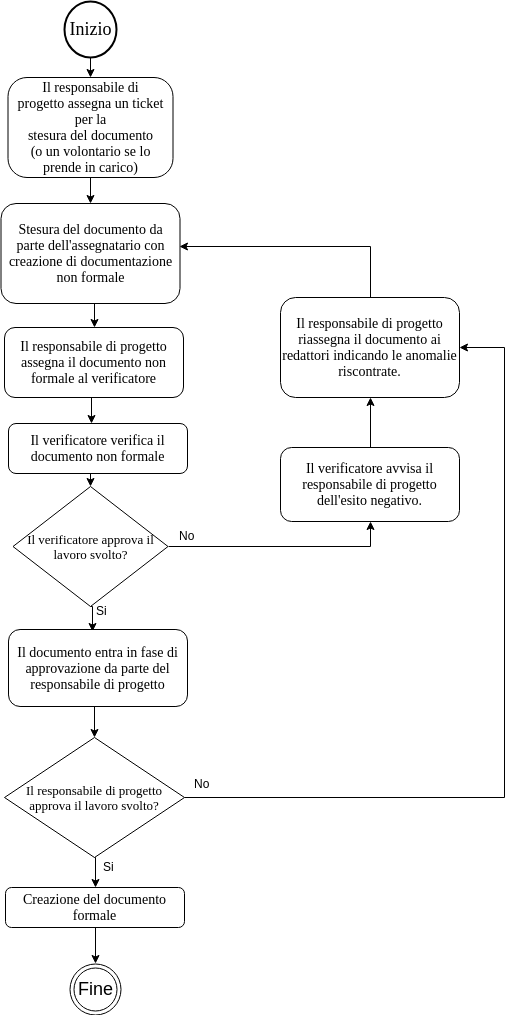
\includegraphics[scale=0.45]{immagini/Dfd.png}
  \caption{Diagramma del ciclo di vita della documentazione}
  \end{center}
\end{figure}

\newpage
\subsubsection{Separazione tra documenti interni e esterni}
I documenti formali redatti dal gruppo Cyber13 rientreranno tassativamente in una delle seguenti categorie (mutuamente esclusive):
    \begin{itemize}
        \item \textbf{Documenti interni} : Documenti ad uso esclusivo del team Cyber13, redatti in lingua Italiana.
        \item \textbf{Documenti esterni}: Documenti che verranno condivisi anche con il proponente e i committenti. Nel caso di documenti utili per il \citgl{deploy}  del software o per il loro utilizzo da parte degli utenti finali, dovranno essere redatti in lingua inglese.
    \end{itemize}

\subsubsection{Nomenclatura dei documenti}
Per quanto riguarda il nome dei documenti formali essi verranno nominati  attraverso la dicitura "NomeDocumento", senza spazi e con lettere maiuscole all'inizio di ogni parola, seguita dalla versione, nella forma: "NomeDocumento\textunderscore vX.Y.Z.estensione". \\
Per quanto riguarda i verbali (interni ed esterni) si seguirà una particolare nomenclatura, descritta nella sezione 4.1.4.3.
        
    \paragraph{Versioni di un documento} 
    ~\\
    Il numero di versione è indicato tramite il carattere ‘v’ seguito da un numero, da un punto, da un numero, da un punto e un numero: vX.Y.Z.
    Ogni volta che si inserisce una modifica nell’omonimo diario, va assegnato un nuovo numero di versione, in modo coerente con le seguenti regole:
                 \begin{itemize}
                    \item Quando verrà creato un documento avrà necessariamente il numero di versione ‘v0.0.1’.
                    \item \textbf{X}: Rappresenta il numero di pubblicazioni ufficiali del documento (quindi ogni qualvolta il documento superi con esito  positivo la fase di approvazione). Ad ogni nuova pubblicazione del documento i valori Y e Z vengono azzerati e quello di X incrementato di uno.
                     \item \textbf{Y}: Rappresenta  il  numero  di  verifiche  eseguite sul documento. L'incremento dell'indice Y implica l'azzeramento del valore dell'indice Z;
                    \item \textbf{Z}: Rappresenta il numero di modifiche effettuate al documento durante il suo sviluppo.
            \end{itemize}
    \paragraph{Formato dei file}
    ~\\
    I documenti sono redatti attraverso lo strumento Latex, pertanto ogni documento si trova nel formato .tex durante il suo sviluppo. Dopo il superamento della fase di approvazione del documento da parte del Responsabile viene il documento viene esportato in formato PDF.
         
\subsubsection{Documenti correnti}
Di seguito si presentano i documenti formali, classificati per appartenenza (interno o esterno) consegnati:
    \begin{itemize}
        \item \textbf{Analisi dei Requisiti}: Uso esterno, sigla (AdR).\\
              Documento per esporre e scomporre i requisiti del progetto contenente i
              \citgl{casi d’uso}
               relativi  al  prodotto  e  diagrammi  di  interazione  con  l’utente.   Viene scritto dagli Analisti dopo aver analizzato il capitolato e interagendo con il Proponente in riunioni esterne.
        \item \textbf{Glossario}: Uso esterno, sigla (GL). \\
              Documento per raccogliere le definizioni dei termini o concetti che saranno usati nei documenti formali per facilitarne la comprensione.
        \item \textbf{Piano di Progetto}: Uso esterno, sigla (PdP). \\
              Documento  per  l’analisi  e  la  pianificazione  della  gestione  delle  risorse  di tempo e umane.
        \item \textbf{Piano di Qualifica}: Uso esterno, sigla (PdQ). \\
              Documento per descrivere standard e obiettivi che il gruppo dovrà raggiungere per garantire la qualità di prodotto e processo.
        \item \textbf{Studio di Fattibilità}: Uso interno, sigla (SdF).\\
              Documento per indicare le riflessioni, punti di forza e caratteristiche sfavorevoli per ogni capitolato proposto sulla base dei quali il gruppo ha fatto la sua scelte.
        \item \textbf{Norme di Progetto}: Uso interno, sigla (NdP).\\
              Documento per mostrare le direttive e gli standard utilizzati all’interno del gruppo di lavoro Cyber13 per lo sviluppo del progetto.
    \end{itemize}

\subsubsection{Formattazione dei documenti}
     \paragraph {Strutturazione dei file}
     ~\\
     Ogni documento formale si deve attenere alla seguente strutturazione dei contenuti:
        \begin{itemize}
            \item \textbf{Frontespizio}: Si tratta della prima pagina dei documenti formali, conterrà le seguenti informazioni (in ordine dall'alto verso il basso):
                \begin{itemize}
                    \item Intestazione: "Università degli Studi di Padova";
                    \item Logo del gruppo: Centrato;
                    \item Titolo del documento: Centrato;
                    \item Nome del gruppo - Nome progetto: In corsivo.
                \end{itemize}
            \item \textbf{Sezione di informazione del documento}: Si trova sempre nella prima pagina del documento e contiene le seguenti informazioni:
                \begin{itemize}
                    \item Versione: Attenendosi alle norme della sezione 3.1.4.2;
                    \item Data Redazione: Seguendo il formato indicato al punto 3.1.6.2 "Formati ricorrenti";
                    \item Responsabile: Nome del responsabile che ha supervisionato il documento;
                    \item Redazione: Nomi dei redattori del documento;
                    \item Verifica: Nomi dei verificatori del documento;
                    \item Approvazione: Nome del responsabile che ha approvato il documento;
                    \item Uso: Interno o esterno;
                    \item Destinatari: A cui è indirizzato il documento;
                    \item Mail di contatto: Mail del gruppo Cyber13.
                \end{itemize}
            \item \textbf{Diario delle modifiche}: Tabella inserita nella seconda pagina del documento. Ha lo scopo di riepilogare l'elenco delle modifiche che sono state apportate al documento nel corso del processo di redazione. L'assegnamento delle versioni si attiene alle norme indicate nella sezione 3.1.4.2 "Versioni del documento".
            Il diario è una tabella ordinata in modo decrescente secondo la data della modifica e, di conseguenza, il numero di versione. Si adotta questo stile per focalizzare gli ultimi cambiamenti poiché trattati nelle prime righe della tabella.
            Ogni riga del diario dovrà contenere i seguenti elementi nell'esatto ordine in cui sono indicati:
                \begin{itemize}
                    \item Versione del documento;
                    \item Data della versione;
                    \item Descrizione delle modifiche apportate;
                    \item Autore delle modifiche apportate;
                    \item Ruolo dell'autore delle modifiche;
                \end{itemize}
            \item \textbf{Indice delle sezioni}: Gli indici hanno lo scopo di riepilogare e dare una visione macroscopica della struttura del documento. Permettono quindi di rintracciare i contenuti tramite una gerarchia. \\
            Ogni documento, esclusi i verbali, dovrà essere corredato dall'indice dei contenuti. 
            Esso sarà posizionato dopo il diario delle modifiche. Se sono presenti tabelle o immagini all'interno del documento, l’indice dei contenuti sarà seguito dalla lista delle tabelle e poi dalla lista delle figure.
            \item \textbf{Elenco delle tabelle}: Vengono indicate tutte le tabelle inserite all'interno del documento.
            \item \textbf{Elenco delle figure}: Vengono indicate tutte le figure inserite all'interno del documento.
            \item \textbf{Introduzione}: Sezione sempre presente nei documenti che ne chiarifica:
                \begin{itemize}
                    \item Scopo del documento;
                    \item Scopo del prodotto;
                    \item Riferimenti: normativi e informativi.
                \end{itemize}
            \item \textbf{Contenuto del documento}: Le restanti pagine del documento sono interamente occupate dal contenuto dello stesso. In ogni pagina, esclusa il frontespizio, devono comparire i seguenti elementi:
                \begin{itemize}
                    \item Logo del team: Dovrà comparire, nell’intestazione della pagina, il logo del gruppo Cyber13. Tale logo sarà posizionato a sinistra.
                    \item Sezione corrente: Il numero e il nome della sezione in cui ci si trova dovranno essere presenti nell'intestazione. Tali elementi saranno posizionati a destra;
                    \item Nome del documento: A piè di pagina, a sinistra, deve apparire il nome del documento completo di versione.
                    \item Numero di pagina: A piè di pagina, a destra, deve comparire il numero della pagina espresso nella seguente notazione: "Pagina x di n", dove x è la pagina corrente e n il numero di pagine totali.
                \end{itemize}
        \end{itemize}
        
     \paragraph{Norme tipografiche}
     ~\\
        \begin{itemize}
            \item \textbf{Virgolette}: Alte singole ’ ’ per singolo carattere,  alte doppie ” ” per racchiudere stringhe mentre parentesi angolari <<  >> per racchiudere citazioni.
            \item \textbf{Parentesi}: Tonde  per  descrivere  esempi  e  fornire  sinonimi  o  precisazioni, quadre per rappresentare uno \citgl{standard} \citgl{ISO}, uno stato relativo a un
            \citgl{ticket}
             o un riferimento ad un codice definito all'interno del documento stesso.
            \item \textbf{Punteggiatura}: Ogni  segno  di  punteggiatura  deve  essere  seguito  da  uno spazio e non avere spazi precedenti al segno stesso;
            \item \textbf{Stile del testo}:
                \begin{itemize}
                    \item Corsivo: Per dare enfasi ad una parola, un concetto o per indicare il nome di un
                    termini di glossario e nomi di  documenti.
                    \item Grassetto: Per i titoli, sottotitoli ed elementi di elenchi e liste di definizione di primo livello.
                    \item Azzurro: Per indicare dei collegamenti ipertestuali.
                \end{itemize}
            \item \textbf{Elenchi}: La prima parola di ogni punto appartenete a un elenco inizierà con la lettera maiuscola. In caso di elenchi di definizioni, al termine da definire seguiranno i ’due punti’ (:)  successivamente vi sarà la sua descrizione. Al termine della descrizione dell'elemento si inserirà il carattere ’punto e virgola’ (;) nel caso di definizione semplice, mentre il carattere 'punto' (.) al termine di una definizione complessa (più di un periodo).
            Per l’ultimo elemento della lista si userà sempre il carattere ’punto’ (.);
            \item \textbf{Formati ricorrenti}:
                \begin{itemize}
                    \item Date: Scritte con lo standard YYYY-MM-DD dove YYYY indica l’anno, MM il mese e DD il giorno;
                    \item Orari: Scritti nel formato 24h.
                \end{itemize}
            \item \textbf{Componenti grafiche}:
                \begin{itemize}
                    \item Immagini: I formati ammessi sono PNG o JPG;
                    \item Tabelle: Devono rispettare lo stile del \citgl{template} \citgl{Latex} realizzato.
                \end{itemize}
        \end{itemize}


\subsubsection{Ambiente}
La stesura dei documenti deve essere effettuata utilizzando il \citgl{linguaggio di markup}
\citgl{LaTeX} e l’ambiente \citgl{Overleaf} con dizionario italiano ed inglese installati.



\subsection{Qualità}
     \subsubsection{Scopo}
Ivi sono descritte le norme alle quali i componenti del gruppo devono sottostare in sede di redazione del \PdQ.


\subsubsection{Aspettative}
Il gruppo desidera redarre il documento \PdQ in modo coerente con quanto riportato nelle norme ivi indicate. 



\subsubsection{Classificazione dei processi}
La qualità del lavoro è garantita dalla suddivisione di quest'ultimo in vari processi, riportati all'interno del Piano di Qualifica.\\
Ad occuparsi di tale suddivisione sono gli Amministratori, che dovranno rispettare la seguente notazione: \\
    \begin{center}
        PROC[num]
    \end{center}
Dove num è un numero positivo, intero di quattro cifre che identifica univocamente il determinato processo. La numerazione parte da "0001".

\subsubsection{Classificazione delle metriche}
La rilevazione della qualità del lavoro è effettuata dagli amministratori attraverso metriche riportate nel \PdQ. Onde evitare ambiguità le metriche dovranno seguire la seguente notazione:
    \begin{center}
        M[categ][sottocateg][num]
    \end{center}
All'interno della quale:
    \begin{itemize}
        \item \textbf{categ}: Indica la categoria della metrica riferendosi a prodotti, processi o test. Può assumere i seguenti valori:
            \begin{itemize}
                \item PROC: Per indicare i processi;
                \item PROD: Per indicare i prodotti;
            \end{itemize}
        \item \textbf{sottocateg}: Indica la sotto-categoria della metrica, se esiste, in caso contrario non è presente.
            \begin{itemize}
                \item Per quanto riguarda la categoria PROC, solo nel caso in cui si tratti di processi di test, possono assumere i seguenti valori:
                    \begin{itemize}
                        \item TA: per indicare tutti i tipi di test
                        \item TM: per indicare i test di modulo
                        \item TH: per indicare i test ad alto livello
                    \end{itemize}
                \item Per quanto riguarda la categoria PROD, possono assumere i seguenti valori:
                    \begin{itemize}
                        \item D: per indicare i documenti;
                        \item S: per indicare il software.
                    \end{itemize}
            \end{itemize}

        \item \textbf{num}: Numero positivo, intero di quattro cifre che identifica univocamente la determinata metrica. La numerazione parte da "0001".
    \end{itemize}

\subsubsection{Procedure}
L'implementazione di metriche tramite procedure verrà studiato con l'avanzare del progetto.

\subsubsection{Metriche per la qualità di processo}
Di seguito sono spiegate nel dettaglio le metriche utilizzate per valutare la qualità dei processi.

\paragraph{M[PROC][0001] - Schedule Variance} ~\\Indica a che livello di avanzamento del progetto rispetto alla pianificazione delle attività.
~\\\\
\centerline{SV = BCWP - BCWS}
\\\\dove BCWP indica le attività svolte e BCWS le attività che dovrebbero essere state svolte finora.

\paragraph{M[PROC][0002] - Budget Variance}
~\\Indica se attualmente si è speso meno o più di quanto previsto.
~\\\\
\centerline{BV = BCWS - ACWP}
\\\\dove BCWS indica il costo pianificato delle attività svolte ad una certa data e ACWP indica il costo effettivo delle attività svolte a tale data.

\paragraph{M[PROC][0003] - Rischi non individuati}
~\\Indice del numero di rischi non individuati nella fase di analisi: è indicato con un numero intero incrementato partendo da zero per ogni rischio rilevato che non fosse stato individuato precedentemente in fase di analisi dei rischi. Viene resettato all'inizio di ogni fase di progetto.

\paragraph{M[PROC][0004]: Numero campi dati per classe}
~\\Indice del numero di campi definiti in una classe. Un numero eccessivo di campi dati rischia di rendere la classe poco specializzata e indica una cattiva progettazione.

\paragraph{M[PROC][0005] - Metodi per classe}
~\\Indice del numero di metodi definiti in una classe.

\paragraph{M[PROC][0006] - Parametri per metodo}
~\\Indice del numero di parametri definiti in un metodo. Un numero eccessivo di parametri per metodo potrebbe sovraccaricare lo \citgl{stack} e comprometterne la funzionalità.

\paragraph{M[PROC][0007]: Grado di instabilità}
~\\È un modo per misurare l'instabilità delle componenti di un sistema, in particolare la possibilità di effettuare modifiche ad un elemento del sistema senza influenzarne altri all'interno dell'applicazione. Questo risultato dipende dall'indice afferente (numero di classi esterne dipendenti da quelle interne) ed efferente (numero di classi interne dipendenti da quelle esterne).
    \\\\
    \centerline{I=${\displaistyle({\frac{Ce}{Ca+Ce}})*100}$}
    \\\\
    dove Ce è indice efferente e Ca è indice afferente.

\paragraph{M[PROC][0008] - Complessità Ciclomatica}
~\\Indica la complessità di funzioni, moduli, metodi o classi di un programma contando il numero di cammini linearmente indipendenti attraverso il grafo di controllo di flusso.

\paragraph{M[PROC][0009] - Linee di codice per linee di comando}
~\\Indica la percentuale di linee di commento presenti all'interno del codice sorgente.
\\\\
\centerline{P = ${\displaystyle({\frac {Nc}{Nsloc}})*100}$}
\\\\dove Nc è il numero di linee di commento e Nsloc è il numero di linee di codice prodotte.

\paragraph{M[PROC][0010] - Halstead Difficulty per-function}
~\\Misura il livello di complessità di una funzione.
\\\\
\centerline{DIF = ${\displaystyle({\frac {UOP}{2}})*{\frac {OD}{UOD}}}$}
\\\\dove UOP è il numero di operatori distinti, OD è il numero totale di operandi e UOD è il numero di operandi distinti.

\paragraph{M[PROC][0011] - Halstead Volume per-function}
~\\Indica la dimensione dell'implementazione di un algoritmo basandosi sul numero di operazioni eseguite e sugli operandi di una funzione.
\\\\
\centerline{VOL = (OP+OD)* ${\log_2 (UOP+UOD)}$}

\\\\dove OP è il numero totale di operatori, OD è il numero totale di operandi, UOP è il numero di operatori distinti e UOD è il numero di operandi distinti.

\paragraph{M[PROC][0012] - Halstead Effort per-function}
~\\Rappresenta il costo necessario per scrivere il codice di una funzione.
\\\\
\centerline{E = DIF*VOL}
\\\\dove DIF indica l'Halstead Difficulty e VOL è l'Halstead Volume.

\paragraph{M[PROC][0013] - Indice di manutenibilità}
~\\Permette di stabilire quanto sarà semplice mantenere il codice prodotto.
\\\\
\centerline{MI = 171-3.42*ln(aveE)-0.23*ln(aveV)-1616.2*ln(aveLOC)}
\\\\dove aveE è l'Halstead Effort medio per modulo, aveV è la complessità ciclomatica media per modulo, e aveLOC è il numero medio di linee di codice per modulo.

\paragraph{M[PROC][TM][0001] - Percentuale di codice coperto da test}
~\\Indica il rapporto tra linee di codice per le quali è previsto un test di verifica su linee di codice totale in percentuale.
\\\\
\centerline{PLcc = ${\displaystyle({\frac {Lcc}{Lct}})}$*100}
\\\\dove Lcc indica linee codice coperte e Lct le linee totali di codice.

\paragraph{M[PROC][TM][0002] - Percentuale di test passati}
~\\Indica il rapporto tra i test passati e i test totali nella fase di sviluppo.
\\\\
\centerline{PTp = ${\displaystyle({\frac {Tp}{Tt}})}$*100}
\\\\dove Tp indica i test passati e Tt i test totali.

\paragraph{M[PROC][TM][0003] - Percentuale di test non passati}
~\\Indica il rapporto tra i test non passati e i test totali nella fase di sviluppo
\\\\
\centerline{PTnp = ${\displaystyle({\frac {Tnp}{Tt}})}$*100}
\\\\dove Tnp indica i test non passati mentre Tt sono i test totali.

\subsubsection{Metriche per la qualità di prodotto}
Di seguito sono spiegate nel dettaglio le metriche utilizzate per valutare la qualità di prodotto.

\paragraph{Metriche per i documenti}
\subparagraph{M[PROD][D][0001]: Indice di \citgl{Gulpease}}
~\\È un indice di leggibilità per la lingua italiana, con il vantaggio di contare le singole lettere e non le sillabe per definire la lunghezza delle parole. 
L'indice prende in considerazione la lunghezza delle parole e la lunghezza delle frasi rispetto al numero totale delle lettere. Come descritto nella seguente formula, restituisce poi un valore che indica l'indice di difficoltà della leggibilità del testo.
\\\\
\centerline{ ${\displaystyle 89+{\frac {300*(numero\ delle\ frasi)-10*(numero\ delle\ lettere)}{numero\ delle\ parole}}}$}
\\\\ Risultati:
\begin{itemize}
    \item Minore di 80: difficile da leggere per chi ha licenza elementare;
    \item Minore di 60: difficile da leggere per chi ha licenza media;
    \item Minore di 40: difficile da leggere per chi ha un diploma superiore.
    \end{itemize}
Ai fini di rendere il testo il più comprensibile possibile, si è deciso di porre importanza anche ad un'analisi diretta da parte di una persona, in quanto l'indice di leggibilità fornito dalla formula sopra riportata non garantisce un buon testo sotto tutti gli aspetti ritenuti importanti. Uno dei motivi che ha spinto il gruppo a questa scelta è dato dal fatto che un risultato considerato non buono secondo l'indice di Gulpease, potrebbe essere conseguenza di un testo con frasi complesse utilizzate per non ricadere in contenuti poco formali; inoltre il risultato non dà informazioni sulla logica del contenuto.\\
Per calcolare l'indice di Gulpease il gruppo ha tenuto conto solo dei contenuti testuali informativi, tralasciando contenuti come indice, intestazione e tabelle.

\subparagraph{M[PROD][D][0002]: Errori ortografici}
~\\\citgl{Overleaf}, l'editor utilizzato per redigere la documentazione, fa uso di un correttore ortografico per mettere in evidenza gli errori di ortografia. Sarà compito del Verificatore correggerli attraverso l'uso di tale strumento.

\paragraph{Metriche per il Software}
\subparagraph{M[PROD][S][0001]: Copertura requisiti obbligatori}
~\\Una volta eseguita l'analisi dei requisiti, essi vengono organizzati in unità di dimensioni gestibili e quelli obbligatori messi in evidenza. Tale metrica indica la percentuale di requisiti obbligatori implementati fino a un dato momento. La formula che la misura è dunque:
    \\\\
    \centerline{CRo = ${\displaystyle{\frac {NRoS}{NRoT}}*100}$}
    \\\\
dove NRoS è il numero dei requisiti obbligatori soddisfatti e NRoT è il numero dei requisiti obbligatori totali

\subparagraph{M[PROD][S][0002]: Copertura requisiti accettati}
~\\Una volta eseguita l'analisi dei requisiti, essi vengono organizzati in unità di dimensioni gestibili e una parte di essi viene identificata come accettati ma non obbligatori. Tale metrica indica la percentuale di implementazione di questi requisiti fino a un dato momento. La formula che la misura è dunque:
    \\\\
    \centerline{CRa = ${\displaystyle{\frac {NRaS}{NRaT}}*100}$}
    \\\\
dove NRaS è il numero dei requisiti accettati che sono stati soddisfatti e NRaT è il numero totale dei requisiti accettati.

\subparagraph{M[PROD][S][0003]: Accuratezza rispetto alle attese}
~\\In fase di testing tale metrica misura la percentuale dei test che hanno restituito i risultati attesi. La formula è la seguente:
    \\\\
    \centerline{AC = ${\displaystyle (1-{\frac {NTf}{NTt}})*100}$}
    \\\\
dove NTf è il numero di test case falliti e NTt è il numero di test case totali.

\subparagraph{M[PROD][S][0004]: Densità di \citgl{failure}}
~\\Rappresenta un dato opposto a quello dell'Accuratezza rispetto alle attese. Indica infatti la percentuale di test conclusi con un esito di failure, quindi negativo, rispetto al totale di test eseguiti.
    \\\\
    \centerline{DF=${\displaystyle({\frac {Nfr}{Nte}})*100}$}
    \\\\
dove Nfr indica il numero di failure rilevati e Nte il numero di test case eseguiti.
    
\subparagraph{M[PROD][S][0005]: Blocco di operazioni non corrette}
~\\È un valore espresso in percentuale che indica il livello di funzionalità con cui si gestiscono correttamente i fault.
    \\\\
    \centerline{BNC=${\dispalystyle({\frac{Nfe}{Non}})*100}$} Nfe: numero di failure evitati durante i test;
    Non: nunmero di test case eseguiti che prevedono l'esecuzione di operazioni non corrette.
    \\\\
   

\subparagraph{M[PROD][S][0006]: Tempo di risposta}
~\\Consiste nel tempo che intercorre tra la domanda al software per una precisa funzionalità e il risultato restituito all'utente.
    \\\\
    \centerline{TR=${\dispalystyle{\frac{\sum_{k=1}^N Tk}{n}}}$}
    \\\\
dove a partire dalla richiesta di n funzionalità, Tk è il tempo trascorso tra una richiesta k per una determinata funzionalità e il termine delle operazioni necessarie a dare seguito a tale richiesta.

\subparagraph{M[PROD][S][0007]: Comprensibilità delle funzioni offerte}
~\\Consiste nella percentuale di operazioni comprese nell'immediato senza il bisogno di consultare il manuale.
    \\\\
    \centerline{CFC=${\displaystyle({\frac{Nfc}{Nfo}})*100}$}
    \\\\
dove Nfc è il numero di funzionalità comprese dall'utente e Nfo è il numero di funzionalità offerte ad esso offerte.

\subparagraph{M[PROD][S][0008]: Facilità di apprendimento delle funzionalità}
~\\Indica il tempo, misurato in minuti, utilizzato dall'utente per apprendere nello specifico una determinata funzionalità e il modo di utilizzarla correttamente.

\subparagraph{M[PROD][S][0009]: Utilizzo effettivo delle funzionalità}
~\\Percentuale che indica il livello di apprezzamento dell'utente rispetto alle funzionalità offerte dall'applicazione.
     \\\\
    \centerline{PA=${\displaystyle({\frac{Nfu}{Nfo}})*100}$}
    \\\\
dove Nfu è il numero funzionalità utilizzate dall'utente e Nfo è il numero funzionalità offerte dall'app.

\subparagraph{M[PROD][S][0010]: Capacità di analisi di failure}
~\\Rapporto, espresso in percentuale, delle failure di cui si conosce la causa rispetto al numero totale di failure attualmente rilevate.
    \\\\
    \centerline{CF=${\displaystyle({\frac{Nfi}{Nft}})*100}$}
    \\\\
dove Nfi è il numero di failure di cui si è identificata la causa e Nft è il numero di failure totali trovate.

\subparagraph{M[PROD][S][0011]: Impatto delle modifiche}
~\\
Dato il numero di failure risolte, questo indice calcola, in percentuale, il rapporto tra quante di esse hanno generato nuove failure in seguito alla loro risoluzione e il loro numero totale.
    \\\\
    \centerline{IM=${\displaistyle({\frac{Nfg}{Nfr}})*100}$}
    \\\\
dove Nfg è il numero di failure generanti (che generano altre failure) e Nfr è il totale di failure risolte.

\subparagraph{M[PROD][S][0012]: Rapporto linee di commento su linee di codice}
~\\Si considera di grande importanza la presenza di commenti che descrivono il codice, in quanto aumentano la leggibilità e l'intelligibilità dello stesso e ne favoriscono la manutenzione, soprattutto in previsione di interventi di più persone.
    \\\\
    \centerline{RLC=${\displaistyle({\frac{Nlcom}{Nlcod}})*100}$}
    \\\\
  dove Nlcom è il numero di linee di commenti e Nlcod è il numero di linee di codice

\subparagraph{M[PROD][S][0013]: Versioni di Android supportate}
~\\È considerato prioritario il supporto delle versioni più recenti del sistema operativo Android, tuttavia è considerato migliorativo un numero maggiore di versioni supportate dall'applicazione.

\subparagraph{M[PROD][S][0014]: Copertura del framework \citgl{Octalysis}}
~\\Il prodotto include funzionalità che seguono i principi del framework di \citgl{gamification} Octalysis.
\\Per misurare la distribuzione di tali funzionalità vengono contate per ogni \citgl{Core Drive} quante appartengono ad ognuno di essi, e rapportati i valori su una scala da 0 a 10. Nel \PdQ{} sono definiti i valori accettabili per ciascun Core Drive. Per la visualizzazione grafica della distribuzione delle funzionalità viene utilizzato il software online Octalysis Tool.
\\Per una breve panoramica sulla gamification e sul framework Octalysis fare riferimento al paragrafo 3.3.3 del \PdQ.
     
\subsection{Configurazione}
     \subsubsection{Scopo}
Nella seguente sezione sono descritte le direttive riguardanti la configurazione degli strumenti di condivisione attraverso i quali sviluppare il materiale da consegnare.



\subsubsection{Aspettative}
Il gruppo si attende alle seguenti norme al fine di condividere tra i vari membri del team il materiale da consegnare in modo ordinato e tracciabile.




\subsubsection{Controllo di versione}
\paragraph{Descrizione}
~\\Si è scelto l'utilizzo della tecnologie Git per la raccolta e la condivisione dei file di documentazione e file non formali, opportunamente organizzati in \citgl{repository} separati.

\paragraph{Struttura delle repository}
~\\Durante la fase di RR son state create due cartelle, una contenente i file non formali chiamata "non formali" e una contenente la documentazione denominata "Documentazione" dove al suo interno è stata creata la cartella "RR" contenente i file di questa fase, organizzati secondo la seguente struttura:
\begin{itemize}
    \item \textbf{Documenti interni}
    \begin{itemize}
        \item Studio Di Fattibilità;
        \item Norme Di Progetto;
        \item Verbali interni.
    \end{itemize}
    \item \textbf{Documenti esterni}
    \begin{itemize}
        \item Piano di Progetto;
         \item Piano di Qualifica;
        \item Analisi dei Requisiti
        \item Glossario;
        \item Verbali esterni.
    \end{itemize}
\end{itemize}
All'interno delle cartelle son presenti i file finali in formato PDF  mentre i file \citgl{LaTex} divisi in sezioni con relativo diario modifiche restano salvati su un account condiviso da tutti i membri del gruppo sulla piattaforma \citgl{Overleaf}.
\paragraph{Branch}
~\\
Per il momento si è deciso di non fare uso dei \citgl{branch} in quanto per lo sviluppo della documentazione da presentare in fase RR si è stabilito di contenere tutto nel master branch. Successivamente verrà creato un branch per ogni membro del gruppo per la gestione del codice in parallelo in uno stesso documento.
\paragraph{Aggiornamento della repository}
~\\
\begin{itemize}
    \item Dare il comando ”git pull” per aggiornare il repository locale sulla base delle modifiche presente in remoto.
    \item Nel caso in cui si verifichino dei conflitti:
    \begin{itemize}
        \item Dare il comando ”git stash” per accantonare momentaneamente le modifiche apportate.
        \item Dare il comando ”git pull” per ottenere ed applicare i \citgl{commit} mancanti.
        \item Dare il comando ”git stash apply” per ripristinare le modifiche.
    \end{itemize}
    \item Dare il comando ”git add [files]” ,  che aggiungerà i file modificati e quelli nuovi specificati;
    \item Dare  il  comando  ”git  commit”  e  successivamente  riassumere  le  modifiche effettuate, in caso sia utile si può aggiungere un messaggio esteso di descrizione (aggiungendo al comando la dicitura -m "messaggio").
    \item Dare il comando ”git push” per completare l’operazione e fornire le modifiche agli altri membri del gruppo.
    
\end{itemize}

\subsubsection{Strumenti}

    \begin{itemize}
        \item\textbf{Client git:} 
        Secondo le preferenze dei membri del gruppo vengono usati principalmente due client \citgl{GitKraken} e \citgl{Git Bash}.
        \item\textbf{Server git:}
        Vista la conoscenza preliminare e l'affidabilità di \citgl{Github} si è scelto questo server.
        
    \end{itemize}

    


\subsection{Verifica}
     \subsubsection{Scopo}
Attraverso il processo di verifica si vuole evidenziare ed eliminare la presenza di errori nell'esecuzione degli altri processi per l'intero sviluppo del prodotto, in particolare alla conclusione di ogni incremento.
Questa sezione norma gli strumenti e i metodi che verranno usati per la verifica del codice e dei documenti.
Per quanto riguarda questa fase antecedente alla RR la verifica verterà
essenzialmente su documenti e diagrammi.



\subsubsection{Aspettative}
Un’implementazione del processo di verifica permette di ottenere i seguenti effetti:
    \begin{itemize}
        \item Ottenere un sistema di controllo degli errori non invasivo, efficiente ed efficace;
        \item Stabilire i criteri necessari per la verifica del prodotto;
        \item Sottolineare le problematiche trovate col fine di risolverle.
    \end{itemize}

\subsubsection{Descrizione}
Il processo si divide nei seguenti momenti:
    \begin{itemize}
        \item \textbf{Controllo}: Attraverso le tecniche di analisi statica e analisi dinamica (descritte nelle sezioni successive) si riesce ad
        effettuare un controllo approfondito del codice sorgente e della sua corretta esecuzione;
        \item \textbf{Test}: Esecuzione test sul software.
    \end{itemize}

\subsubsection{Attività}

    \paragraph{Analisi statica}
        ~\\ 
        L’analisi statica è una tecnica di analisi applicabile sia alla documentazione che al codice e permette di effettuare la verifica di quanto prodotto individuando errori ed anomalie.\\
        Vi sono due metodologie per effettuarla:
            \begin{itemize}
                \item \textbf{Walkthrough}: tecnica applicata quando non si sanno le tipologie di errori o problemi che si stanno cercando e quindi prevede una lettura da cima a fondo del codice o documento per trovare anomalie di qualsiasi tipo. Questo metodo risulta essere il più dispendioso in termini di efficienza ma si tratta anche del più semplice da imparare, diventando inevitabilmente il più utilizzato nelle prime fasi del progetto.
                \item \textbf{Inspection}: tecnica da applicare quando si ha idea delle possibili problematiche che si stanno cercando e si attua leggendo in modo mirato il documento o il codice. Questo procedimento risulta molto più veloce del precedente in quanto,
                utilizzando la lista di controllo degli errori e dalle misurazioni effettuate, permette un’analisi più efficace dei punti critici, tralasciando invece le parti senza problematiche.
            \end{itemize}
        
        \paragraph {Analisi dinamica}
        ~\\
        Il processo di analisi dinamica consiste nella realizzazione ed esecuzione di una serie di test di vario tipo sul codice del software.  Questa tecnica non è applicabile per trovare errori nella documentazione. 
        
            \subparagraph{Test}
            ~\\
            Poiché la fase di RR prevede la sola preparazione di documentazione, le norme che regolano l'analisi dinamica verranno definite in seguito.
        

\subsubsection{Strumenti}
    \begin{itemize}
        \item \textbf{Documenti}: Per  quanto  riguarda  la  verifica  ortografica ci si affida allo strumento integrato di Overleaf, attraverso il quale le parole sbagliate vengono segnate in rosso, permettendo un controllo rapido ed efficace.
        
         \item \textbf{Indice Gulpease}: Per il calcolo dell’Indice  di  Gulpease il team ha utilizzato lo strumento disponibile online chiamato \citgl{Farfalla Project};
         
         \item \textbf{Octalysis Tool}: Per una valutazione della qualità degli aspetti relativi alla \citgl{Gamification} si è scelto di utilizzare lo strumento online Octalysis Tool disponibile sul sito del creatore del framework \citgl{Octalysis} Yu-kai Chou.
         
         \item \textbf{Gestione processi e feedback}: Anche per la verifica si è stato scelto di utilizzare il sistema di \citgl{issues} integrato in GitHub.
         
         
    \end{itemize}



\subsection{Validazione}
     \subsubsection{Scopo}
Il processo di validazione ha l’obiettivo di verificare che il prodotto sia conforme
a quanto pianificato e sia abile nel gestire e minimizzare gli effetti degli errori.

\subsubsection{Aspettative}
In questa sezione il gruppo intende sviluppare direttive utili per eseguire correttamente il processo di validazione. 




\subsubsection{Procedure}
I passi per compiere l’attività di validazione sono i seguenti:
    \begin{itemize}
        \item \textbf{Tracciamento}: Tracciamento dei test con rendiconto eseguito dai verificatori;
        \item \textbf{Analisi risultati}: In seguito a seguire il Responsabile di progetto controlla e analizza i report ricevuti sui test decidendo se:
            \begin{itemize}
                \item Accettare la validazione e consegnare i risultati al proponente, informandolo sulle modalità di esecuzione della validazione;
                \item Chiedere la ripetizione di alcuni o tutti i test con ulteriori nuove indicazioni.
            \end{itemize}
    \end{itemize}
                \newpage
            \section{Processi organizzativi}
                \subsection{Processi di coordinamento}
\subsubsection{Scopo}
In questa sezione vengono elencate direttive, linee guida e strumenti che il gruppo dovrà utilizzare a fini organizzativi all'interno dello svolgimento del lavoro.
\subsubsection{Aspettative}
Il gruppo si attende alle seguenti direttive al fine di organizzare, evitando incomprensioni di varia natura, gli incontri tra i componenti.



\subsubsection{Comunicazione}
In questa sezione vengono illustrati i metodi di comunicazione sia tra i membri all'interno del gruppo Cyber13 sia tra il gruppo e le entità esterne, come Committenti e Proponenti.
    \paragraph{Comunicazioni interne}
    ~\\Le comunicazioni interne al gruppo avvengono tramite \citgl{Slack}, strumento di messaggistica nel quale sono stati predisposti dei canali tematici, suddivisi per argomento:
    \begin{itemize}
    \item \textbf{general:} Canale di carattere generale, per coordinare luoghi e orari di ritrovo, scambiare opinioni sul progetto e in generale inviare comunicati che non trovano spazio in alcuno degli altri canali specifici.
    \item \textbf{documentirr:} Canale predisposto per la coordinazione e l'aggiornamento dei lavori del team su tutti i documenti da approntare in vista della RR di Aprile 2019 (si procederà allo stesso modo anche per le fasi successive).
    
    \end{itemize}
    \paragraph{Comunicazioni esterne}
    ~\\Alcune norme regolano anche le comunicazioni con le parti esterne al gruppo Cyber13, nello specifico:
    \begin{itemize}
    \item La proponente GaiaGo rappresentata da Filippo De Pretto, con la collaborazione del quale si definiranno i \citgl{requisiti} che porteranno alla realizzazione del prodotto;
    \item I committenti Prof. Tullio Vardanega e Prof. Riccardo Cardin, ai quali verrà fornita la documentazione richiesta in ciascuna revisione di progetto. 
    \end{itemize}
    \textbf{Comunicazioni esterne scritte}
    ~\\ Le comunicazioni esterne scritte vengono effettuate utilizzando l'indirizzo e-mail del gruppo \url{swe.cyber13@gmail.com} a cui tutti i membri hanno accesso.
    Per comunicare con il Proponente viene utilizzato l'indirizzo e-mail \url{f.depretto@gaiago.com}.
    Anche le comunicazioni con i committenti avvengono esclusivamente tramite l'indirizzo e-mail del gruppo: ogni messaggio deve essere definito da un oggetto chiaro e conciso, così come deve essere il suo contenuto, e rivolgersi ai committenti in modo formale e cortese.
    
\subsubsection{Riunioni}
Le riunioni interne ed esterne al team Cyber13 sono un momento fondamentale per il corretto avanzamento e conclusione del progetto. Alcune regole ne normano quindi l'organizzazione e lo svolgimento.
\\Per ogni riunione viene nominato un Segretario tra i membri del gruppo, il quale garantirà il rispetto dell'ordine del giorno, si occuperà di annotare i punti più importanti discussi e da tali appunti redigerà infine un Verbale di Riunione. Quest'ultimo non è un ruolo fisso, quindi il membro del team che ne ricoprirà la carica potrà variare da riunione a riunione se necessario.
\\Le riunioni che non potranno avere un luogo fisico di ritrovo avverranno in remoto attraverso il programma \citgl{Skype} o lo strumento \citgl{ Google Meet}, secondo quanto concordato preventivamente prima dell'appuntamento.

    \paragraph{Riunioni interne}
    ~\\La partecipazione è ammessa ai soli membri del team Cyber13.
    \\Ordine del giorno, data, ora e luogo della riunione vengono decisi dal Responsabile di progetto, che si occupa anche di approvare il Verbale di Riunione stilato dal Segretario.
    \\I membri del team hanno il dovere di presentarsi in orario all'appuntamento, comunicando eventuali ritardi e partecipando attivamente e costruttivamente alla discussione.
    \\La riunione è considerata valida se almeno 5 dei 6 membri del team sono presenti. In circostanze eccezionali qualora un membro fosse impossibilitato ad essere presente di persona  ma la sua presenza dovesse essere fondamentale per la discussione dell'ordine del giorno, esso potrà prendere parte alla riunione da remoto attraverso uno strumento di videochiamata come Skype o Google Meet.
    
    \paragraph{Riunioni esterne}
    ~\\Prendono parte a queste riunioni i membri del team Cyber13 e la Proponente.
    \\Essendo la sede di GaiaGo a Milano, le riunioni esterne avranno il più delle volte luogo da remoto, attraverso uno strumento quale Skype o Google Meet, deciso di volta in volta prima dell'appuntamento.
    \\Le riunioni esterne cui la Proponente prenderà parte di persona saranno invece effettuate presso la Torre Tullio Levi Civita (ex Torre Archimede), previa disponibilità dei locali.
    \\Come per le riunioni interne, il Verbale di Riunione sarà redatto da un Segretario eletto di volta in volta e sarà approvato in seguito dal Responsabile di Progetto.
    \\Data l'elevata importanza delle riunioni esterne, esse vengono considerate valide anche alla presenza di un singolo membro del team Cyber13 e della Proponente.
    
    \paragraph{Verbale di riunione}
    ~\\Il Segretario eletto di volta in volta si occupa di stilarlo secondo il seguente schema:
    \begin{itemize}
        \item \textbf{Verbale TIPO del DATA:} Il frontespizio del Verbale di Riunione permette di identificarne il TIPO (Interno/Esterno) e la DATA in cui la riunione ha avuto luogo.
        \item \textbf{Diario delle modifiche:} Come definito nella sezione 3.1.6.1.
        \item \textbf{Indice:} Semplice indice dei contenuti del Verbale.
        \item \textbf{Informazioni sulla riunione:} Deve contenere obbligatoriamente le seguenti informazioni:
        \\ \textbf{- Luogo e data della riunione:} ad esempio Padova, 15 Marzo 2019;
        \\ \textbf{- Partecipanti alla riunione:} a partire dai Proponenti/Committenti in caso di Riunione Esterna, seguiti dai nomi dei membri del team Cyber13 presenti elencati in ordine alfabetico.
        \\\\Possono invece considerarsi informazioni facoltative ma utili:
        \\ \textbf{- Ora di inizio e di fine:} scritte nel formato 24h;
        \\ \textbf{- Motivo della riunione:} Illustra in forma riassuntiva i motivi generali della riunione;
        \item \textbf{Ordine del giorno:} Indica attraverso un elenco numerato gli argomenti da discutere così come definiti dal Responsabile di Progetto;
        \item \textbf{Resoconto:} riassunto di quanto discusso in riunione, redatto dal Segretario. Indicherà chiaramente quali punti dell'Ordine del Giorno sono stati effettivamente affrontati, eventuali argomenti discussi che non fossero presenti nell'Ordine del Giorno e le relative decisioni prese.
        \\Il tracciamento delle decisioni prese avverrà attraverso un sistema a codici del tipo VER-DATA.X dove VER significa Verbale, DATA è sostituito con la data della riunione e X è un numero sequenziale che identificherà univocamente la decisione cui si sta facendo riferimento.
    \end{itemize}
    \\\\ \textbf{Nomenclatura e archiviazione dei verbali:} I Verbali di Riunione saranno archiviati con la nomenclatura VER-DATA dove DATA è la data della riunione nel formato YYYY-MM-DD per permetterne un posizionamento semplice e cronologico all'interno della cartella assegnata.
    \\Trattandosi di documenti esterni e ufficiali, verranno archiviati nella cartella di Repository dedicata e saranno redatti in LaTeX.
\subsection{Processi di pianificazione}
\subsubsection{Scopo}
In questa sezione vengono elencate le norme relative ai processi di pianificazione interni al gruppo.
\subsubsection{Aspettative}
Il gruppo si aspetta di organizzare in maniera ottimale ed evitando incomprensioni di varia natura la divisione del lavoro da svolgere. Per fare vengono stabiliti ruoli precisi all'interno del progetto.


\subsubsection{Ruoli di progetto}
Nel corso del progetto ogni componente del team avrà modo di ricoprire a rotazione il ruolo di ognuna delle figure aziendali tipicamente coinvolte nella realizzazione di un software.
\\Tale assegnazione cercherà di distribuire nel modo più omogeneo possibile il tempo che ciascun membro investirà in ogni ruolo, dando in ogni caso priorità alla continuità delle attività già in corso.
\\Il Responsabile di Progetto di turno dovrà inoltre garantire che non si creino situazioni di conflitto di interesse che potrebbero compromettere la qualità del prodotto finale.
    \paragraph{Responsabile di progetto}
    ~\\Il "Responsabile di progetto", o "Project Manager", accentra le responsabilità di scelta e approvazione del gruppo, del quale è anche il rappresentante presso proponenti e committenti.
    \\Si occupa quindi di gestire le risorse umane e di coordinare i membri del team, dell'approvazione dei documenti, della pianificazione e delle relazioni esterne.
    \paragraph{Ammininstratore}
    ~\\L'amministratore è una figura di supporto che si occupa di fornire al team gli strumenti per lavorare in maniera rigorosa e regolamentata.
    \\Tali strumenti consistono nella redazione e attuazione di piani e procedure di Gestione della Qualità, la redazione delle Norme di Progetto, il versionamento e la configurazione dei prodotti.
    \\Pur non essendo sotto sua diretta responsabilità, collabora alla redazione del Piano di Progetto e si assicura che la documentazione sia corretta e verificata.
    \paragraph{Analista}
    ~\\L'analista si occupa di analizzare e capire appieno il dominio del problema per identificarne i requisiti espliciti ed impliciti, e per riconoscere ed evitare gravi problemi di progettazione successivi.
    \\Essendo colui che all'interno del team meglio conosce il problema e i requisiti che la sua realizzazione richiede, esso è coinvolto anche nella definizione degli accordi contrattuali, nella verifica delle implicazioni di costo e qualità, nella realizzazione dello Studio di Fattibilità e dell'Analisi dei Requisiti.
    \paragraph{Progettista}
    ~\\Il progettista si occupa della definizione di una soluzione soddisfacente per tutti gli \citgl{stakeholder}, perseguendo efficienza ed efficacia nella soddisfazione dei requisiti a partire dal lavoro dell'Analista.
    \\In tal senso il progettista conosce e applica soluzioni di lavoro note e ottimizzate (\citgl{Best practice}), e si occupa di organizzare e suddividere il sistema in parti di complessità trattabile, per rendere il lavoro di codifica realizzabile e verificabile.
    \paragraph{Programmatore}
    ~\\Il programmatore si occupa della codifica del progetto, realizzando quindi il prodotto finale attraverso l'implementazione dell'architettura definita dal Progettista.
    \\Il codice prodotto deve essere documentato, versionato e mantenibile secondo le norme fissate.
    \\Si occupa anche della scrittura del Manuale Utente e di realizzare le componenti necessarie alla verifica e alla validazione del codice.
    \paragraph{Verificatore}
    ~\\Il verificatore è coinvolto in ogni fase del progetto. Il suo compito è appunto quello di verificare la conformità dei prodotti ai requisiti fissati di funzionalità e qualità.
    \\Il suo coinvolgimento è richiesto in ogni fase poiché deve accertarsi che ad ogni attività di processo eseguita non siano stati introdotti errori.
    \\Attraverso la redazione di un Piano di Qualifica si occupa di illustrare le verifiche effettuate sul progetto e i relativi esiti, secondo quanto previsto dal Piano di Progetto.
    \paragraph{Rotazione dei ruoli}
    ~\\Per assicurare un buon esito del progetto e allo stesso tempo assicurare una rotazione dei ruoli assegnati a ciascun membro del gruppo durante la sua realizzazione, sono necessarie alcune semplice regole:
    \begin{itemize}
        \item Considerare impegni e interessi di ogni singolo membro del gruppo;
        \item Evitare conflitti di interesse, in particolare evitare che un ruolo assegnato ad un membro del gruppo comporti la verifica di lavoro svolto in precedenza dallo stesso mentre ricopriva un altro ruolo all'interno della stessa fase dello sviluppo.
        \item Garantire che al cambio di ruolo il nuovo assegnatario venga posto nelle migliori condizioni di lavoro possibile. In tal senso il precedente assegnatario deve assicurarsi di non lasciare al nuovo criticità da lui non gestibili. Inoltre si occuperà di lasciargli al nuovo una lista di consigli e procedure utili in un documento interno informale.
        \item Garantire che ciascun membro ricoprirà di volta in volta il ruolo a lui assegnato in modo esclusivo: ciascuno dovrà occuparsi di quanto è di sua competenza, senza interferire o incrociare incarichi e responsabilità.
    \end{itemize}
    \subsubsection{Ticketing}
    
    \paragraph{Task list}
    ~\\Lo svolgimento del progetto prevede la suddivisione del modello di sviluppo in varie fasi. Le attività da svolgere in una fase sono contenute in una \citgl{task board}.Il responsabile ha il compito di creare le task board per ogni fase del modello su \citgl{GitHub}, utilizzando il nome "X", dove X identifica in modo significativo la sezione di progetto cui si riferisce. Per esempio, per quanto riguarda i documenti, X segue la nomenclatura indicata nella sezione 3.1.4.1. 
    \paragraph{Task}
     ~\\Ogni singola \citgl{task} viene creata o approvata dal Responsabile di progetto ed è caratterizzata da un titolo significativo per la componente di progetto cui si riferisce. 
    \paragraph{Ticket}
    ~\\Il \citgl{ticket} sono lo strumento attraverso cui viene gestito il ciclo di vita del task, dalla sua definizione, alla sua assegnazione ad uno o più membri del gruppo, alla sua implementazione, verifica, approvazione e chiusura.
     L'assegnazione del \citgl{ticket} ad uno specifico membro del gruppo può avvenire secondo due modalità:
    \begin{itemize}
        \item \textbf{Direttamente}: L'assegnazione del task è già noto al momento della creazione dello stesso. In questo caso il \citgl{ticket} viene assegnato direttamente allo specifico componente del gruppo da parte del Responsabile di progetto.
        \item \textbf{Indirettamente}: Nel caso in cui un membro non è presente agli incontri oppure il lavoro che richiede una \citgl{task} è impegnativo, può non essere possibile assegnare direttamente un ticket ad un componente del gruppo. In questo caso il membro non presente è obbligato a controllare la sezione \citgl{issues} presente su \citgl{GitHub} dove troverà il lavoro da svolgere. Questi tasks inoltre possono essere assegnati qualora il componete finisse i \citgl{ticket} a suo carico.
    \end{itemize}

\newpage
    
\subsection{Procedure}
\subsubsection{Creazione e gestione dei task}
Per la creazione di un task si procede nel seguente modo:
\begin{itemize}
    \item Accesso alla task list relativa al progetto di interesse identificata con il nome dello stesso.
    \item Creazione di un nuovo task.
    \item Il Responsabile di Progetto può decidere si suddividerlo in sotto-task da assegnare a membri del gruppo differenti.
\end{itemize}
\subsubsection{Gestione dei ticket}
La vita di ogni ticket viene presentata nel seguente diagramma:

\begin{figure}[h!]
  \begin{center}
  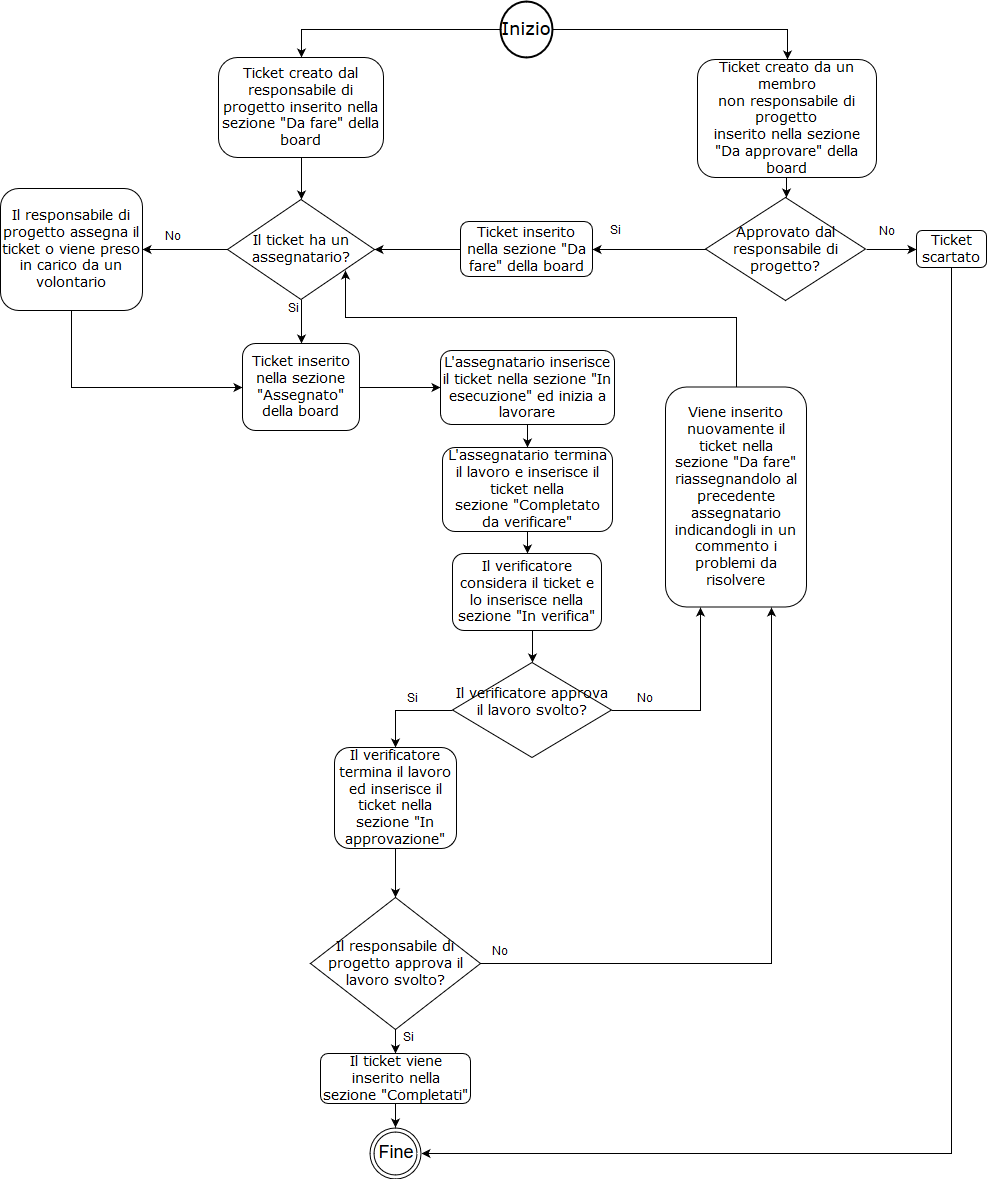
\includegraphics[scale=0.50]{immagini/Dt.png}
  \caption{Diagramma del ciclo di vita di un ticket}
  \end{center}
\end{figure}

\newpage

\subsubsection{Stesura del consuntivo}
L'operazione di stesura del consuntivo viene eseguita dal Responsabile di Progetto nel seguente modo:
\begin{itemize}
    \item Esporta da \citgl{Gantt project} un file in formato \citgl{Microsoft Excel} che indica le ore rendicontate nella fase corrente;
    \item Accede al \citgl{Foglio di Google} presente nel \citgl{Google Drive} associata alla mail del gruppo con relativo template e ne fa una duplicazione;
    \item Inserisce le ore rendicontate nelle apposite celle ottenendo la differenza con quelle preventivate;
    \item Riporta i valori ottenuti nel Piano di Progetto;
    \item Crea una tabella che, elaborando i dati derivanti dalla differenza tra le ore rendicontate e quelle preventivate, trova il budget effettivo rispetto a quello previsto;
    \item Infine con l'elaborazione di questi dati crea una valutazione complessiva del lavoro.
\end{itemize}
Per il periodo che precede la revisione RR ci si ferma al punto 3 senza ricavarne la differenza in quanto le ore preventivate non sono presenti. Successivamente ad ogni revisione sarà aggiornato il Piano di Progetto con i dati ottenuti.


\subsection{Strumenti}
\subsubsection{Pianificazione}
Per la pianificazione la scelta è ricaduta sulla piattaforma GitHub perchè offre la possibilità di organizzare le task di progetto in ticket, da assegnare a uno o più membri ed infine organizzarli in colonne. A tal proposito il gruppo ha deciso di creare varie colonne una per ogni fase del ciclo di vita del ticket in modo da avere un idea chiara sul punto in cui sono i vari membri del gruppo con i relativi compiti.
\subsubsection{Comunicazione}
Per la comunicazione ci si è orientati per l'applicazione di messaggistica \citgl{Slack} apposita per gruppi di lavoro, che offre la possibilità di realizzare canali telematici, in modo da creare comunicazioni specifiche per argomento.
Per le comunicazioni interne al gruppo finora non si ha avuto la necessità di utilizzare strumenti per video chiamate in quanto ci si è organizzati in modo efficiente sugli incontri settimanali. In caso di necessità futura nei si prevede di utilizzare \citgl{Skype} e \citgl{Google Meet} che permettono video chiamate di gruppo.
\subsubsection{Creazione diagrammi di Gantt}
Per la realizzazione di diagrammi di \citgl{Gantt} si è scelto lo strumento \citgl{open source} e  \citgl{multipiattaforma} GanttProject.

\subsubsection{Calcolo del consuntivo}
Gli strumenti a disposizione dal Responsabile di Progetto sono i seguenti:
\begin{itemize}
    \item Fogli Google
    \item GanttProject
\end{itemize}
\item
\subsection{Formazione}
La formazione del personale è da svolgersi autonomamente. I membri del team Cyber13 sono tenuti a studiare individualmente le tecnologie che verranno utilizzate durante lo svolgimento del progetto.\\
La documentazione di riferimento, oltre al materiale precedentemente citato nella sezione 1.4.2 Riferimenti informativi, comprende:
    \begin{itemize}
        \item Documentazione LaTeX: \\
              \url{https://www.latex-project.org}
        \item Documentazione GitHub: \\
              \url{https://github.com}
        \item Documentazione UML: \\
            \url{https://www.math.unipd.it/~tullio/IS-2/Guida_Notazioni_UML-14.pdf}
    \end{itemize}
                \newpage
		    
		\newpage
\end{document}
    